\section{Zielsetzung}
In diesem Versuch wird die Leerlaufspannung und der Innenwiderstand von realen Spannungsquellen bestimmt.

\section{Theorie}
\label{sec:Theorie}
Anders als bei idealen Spannungsquellen, die sich dadurch auszeichnen, ihre eingestellte Spannung $U_\text{Soll}$ an den Klemmen trotz Belastung ohne Verluste aufrecht erhalten zu können, 
sinkt bei realen Spannungsquellen die Klemmenspannung $U_\text{K}$, sobald Verbraucher elektrische Leistung beziehen.
Die Spannung, die an den Klemmen anliegt, ohne dass Verbraucher angeschlossen sind, 
wird als Leerlaufspannung $U_0$ bezeichnet und fällt mit $U_\text{Soll}$ einer idealen Spannungsquelle zusammen.

Zur Beschreibung des Spannungsverlustes wird ein Innenwiderstand $R_\text{i}$ innerhalb der Spannungsquelle eingeführt, der fester Bestandteil einer realen Spannungsquelle ist.
\begin{figure}[ht]
	\centering
  	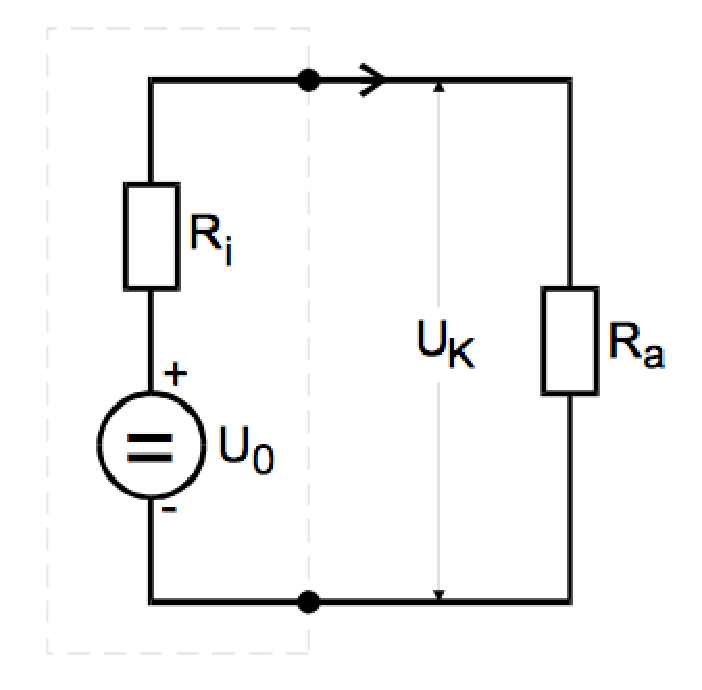
\includegraphics[width=0.4\textwidth]{Bilder/Innenwiderstand}
	\caption{Skizze eines einfachen Schaltkreises mit Ersatzschaltbild der Spannungsquelle. \cite{V301}}
	\label{fig:Innenleben}
\end{figure}
Die reale Spannungsquelle wird der Abbildung \ref{fig:Innenleben} gemäß als ideale Spannungsquelle mit $U_\text{Soll}$ und dem Innenwiderstand $R_\text{i}$ aufgefasst. 
Die Klemmenspannung ist in Reihe nach Spannungsquelle und Innenwiderstand abgreifbar.
Mit der zweiten Kirchhoffschen Regel gilt für die Klemmenspannung
\begin{equation}
	U_\text{k} = U_\text{0} - R_\text{i}\cdot I
	\label{eq:Klemmspannung}
\end{equation}

Die Annahme des Innenwiderstandes hat zur Folge, dass nicht beliebig hohe Leistungen von dem Verbraucher $R_\text{a}$ aufgenommen und ebenfalls nicht beliebig hohe Leistungen von dem Spannungsgerät geliefert werden können. 
Die an den Verbraucher $R_\text{a}$ abgegebene Leistung 
\begin{equation}
N(R_\text{a}) = I^2\cdot R_\text{a}=U_0²\frac{R_\mathup{i}}{\bigl(R_\mathup{i}+R_\mathup{a}\bigr)²}
\label{eq:leistungsanpassung}
\end{equation}
 lässt eine Leistungsoptimierung in $R_\text{a}$ zu. 
Damit existiert für eine gegebene Spannungsquelle mit bekanntem Innenwiderstand $R_\text{i}$ ein optimaler Gesamtwiderstand \\$R_\text{a, optimal}=R_\mathup{i}$ des Verbrauchers,
bei welchem die Leistung maximal wird.
